\documentclass[12pt]{article}

\usepackage{alltt}
\usepackage{epsfig}
\usepackage{pstricks}
\usepackage{xspace}
%\usepackage{makeidx}
\usepackage{index}
%\usepackage{multind}

\makeindex

\newindex{MLbn}{bnx}{bnd}{Index of ML bindings}
\newindex{MLty}{tnx}{tnd}{Index of ML types}

\newcommand{\bnind}[1]{\index[MLbn]{#1}}
\newcommand{\tyind}[1]{\index[MLty]{#1}}


\newlength{\minipagewidth}
\setlength{\minipagewidth}{\textwidth}
\addtolength{\minipagewidth}{-5mm}

\newenvironment{greekenumerate}{\begin{enumerate}
  \renewcommand{\theenumi}{\roman{enumi}}
  \renewcommand{\labelenumi}{(\roman{enumi})}}{\end{enumerate}}

\renewcommand{\t}[1]{\mbox{\tt #1}}
\newcommand{\con}[1]{\mbox{\sf #1}}
\newcommand{\ty}[1]{\mbox{\tt #1}}
\newcommand{\prev}[1]{#1}

\newcommand{\varord}[1]{#1}

\newcommand{\ma}[1]{{{$#1$}}}
\newcommand{\ml}[1]{{\tt #1}}
\newcommand{\id}[1]{#1}

\newcommand{\redonlightgray}[1]%
{\psset{fillcolor=lightgray}\psframebox*[framearc=.3]{\red #1}}

\newcommand{\termbdd}[3]{\mbox{$#1~#2~\mapsto~#3$}}
\newcommand{\globtermbdd}[2]{\mbox{$#1\hspace{0.5mm}\mapsto\hspace{0.5mm}#2$}}
\newcommand{\qq}[1]{\mbox{\tt{`\hspace{-1.3mm}`}}#1\mbox{\tt{`\hspace{-1.3mm}`}}}

\newcommand\termbddty{\texttt{term\_bdd}\xspace}

\newcommand\HOL{HOL\xspace}
\newcommand\Hol{Hol98\xspace}
\newcommand{\mosml}{Moscow~ML\xspace}
\newcommand{\Buddy}{BuDDy\xspace}
\newcommand{\Muddy}{MuDDy\xspace}
\newcommand\HolBuddy{\texttt{HolBddLib}\xspace}

\newcommand\fun{\mbox{\tt{->}}}
\newcommand\turn{{\vdash}}
\newcommand\imp{{\Rightarrow}}
\newcommand\T{\con{T}}
\newcommand\F{\con{F}}

\newcommand{\cond}{\rightarrow}
\newcommand{\els}{\mid}
\newcommand{\Imp}{\Rightarrow}

\renewcommand{\prod}{\mbox{\tt{*}}}
\newcommand{\SP}{~}
\newcommand{\SPP}{~}

\newcommand{\homedir}{\mbox{$\sim$}}

\newcommand{\Turn}{\(\turn\)}
\newcommand{\And}{\(\wedge\)}
\newcommand{\Or}{\(\vee\)}
\newcommand{\Not}{\(\neg\)}
\newcommand{\Forall}{\(\forall\)}
\newcommand{\Exists}{\(\exists\)}
\newcommand{\Mapsto}{\(\mapsto\)}


\parindent 0mm
\parskip 1mm


% ---------------------------------------------------------------------
% Macros for little HOL sessions displayed in boxes.
%
% Usage: (1) \setcounter{sessioncount}{1} resets the session counter
%
%	 (2) \begin{session}\begin{verbatim}
%	      .
%	       < lines from hol session >
%	      .
%	     \end{verbatim}\end{session}   
%
%            typesets the session in a numbered box.
% ---------------------------------------------------------------------

\newlength{\hsbw}
\setlength{\hsbw}{\textwidth}
\addtolength{\hsbw}{-\arrayrulewidth}
\addtolength{\hsbw}{-\tabcolsep}

\newcounter{sessioncount}
\setcounter{sessioncount}{1}

\newcommand\MLSpacing{13pt}
\newenvironment{session}{\begin{flushleft}
 \begin{tabular}{@{}|c@{}|@{}}\hline 
 \begin{minipage}[b]{\hsbw}
 \vspace*{-.5pt}
 \begin{flushright}
 \rule{0.01in}{.15in}\rule{0.3in}{0.01in}\hspace{-0.35in}
 \raisebox{0.04in}{\makebox[0.3in][c]{\footnotesize\sl \thesessioncount}}
 \end{flushright}
 \vspace*{-.45in}
 \begingroup\small\baselineskip\MLSpacing}{\endgroup\end{minipage}\\ \hline 
 \end{tabular}
 \end{flushleft}
 \stepcounter{sessioncount}}

\begin{document}
\thispagestyle{empty}

\hrule height5pt

\begin{flushleft}
{\Huge{\tt HolBddLib} Version 2\\[5mm]
Documentation}
\end{flushleft}

\vspace*{2mm}

\hrule height5pt

\vspace*{1cm}


\noindent{\Large{\bf Mike Gordon}}

\vspace*{5mm}

\today

\vfill

{\setlength{\fboxrule}{0.5mm}
\setlength{\fboxsep}{2mm}
\fbox{
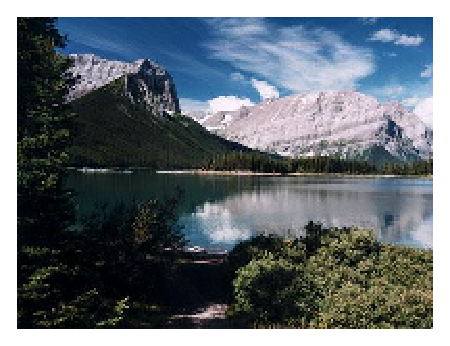
\epsfig{file=kananaskis_small.ps} \raisebox{2.5cm}{\Huge\bf~~~+~} 
\raisebox{0mm}{\epsfig{file=scratchBDD.ps, height=5.3cm, width=3.5cm}}
}}

\vfill

\newpage

\pagenumbering{roman}

\section*{Preface}


The development of {\tt HolBddLib} has gone through two phases
\cite{Gordon:TPHOLs2000}.
The goal of Version~2, described here, is to provide core
infrastructure for building `fully-expansive' or `LCF-style'
combinations of HOL theorem proving and BDD-based symbolic calculation
algorithms, like model checkers.

The first version, Version~1, of {\tt{HolBddLib}} was in some ways more elaborate than Version~2
because it mixed together code from a number of experiments
exploring diffferent styles of linking terms of higher order logic to
BDDs. Version~2 is rigorously based a protected type
of `BDD representation judgements' (analogous to the LCF protected type of theorems)
and provides a fixed set of `inference rules' that link terms to BDDs. All other tools,
such as model checkers, are programmed in ML as `derived rules'.

The primitive rules are in the structure {\tt{PrimitiveBddRules}} and an initial
set of derived rules is in the structure {\tt{DerivedBddRules}}. Currently the only derived rules
are to compute reachable states and find sequences of transitions to states with given properties.
It is hoped to soon add a module checking properties expression
in the modal $\mu$-calculus (and hence CTL).

In {\tt{HolBddLib}} Version~1 there was a function, called
{\texttt{termToBdd}}, that tried to represent a \HOL{} term as a BDD
using a dynamically extendable global table mapping \HOL{} terms to
BDDs.  $\t{TermToBdd}$ constructed the BDD of a term $t$ using any
BDDs of subterms of $t$ that were stored in the global table.
{\tt{HolBddLib}} Version~2 has jettisoned this imperative style based
on a global BDD state in favour of a purely functional rules. Some of
the ideas of BDD tables are likely to return in the future, but as
contexts, similar to HOL simpsets, that are passed functionally,
rather than as a single global state held in references.

{\tt{HolBddLib}} Version~1 only supported a single variable
ordering, held in a global variable map. In Version~2, each
representation judgement carries its own variable ordering, so that local
scopes are possible. For convenience, {\tt{DerivedBddRules}}
provides a way of storing a default variable ordering in a global
variable, but this is just a derived facility, not part of the kernel.

{\tt HolBddLib} uses J{\o}rn Lind-Nielsen's \Buddy{} package as a BDD
engine. The interface from \Buddy{} to Moscow ML, called \Muddy, is
due to Ken Friis Larsen and Jakob Lichtenberg, and is described in Part~\ref{muddy}.
{\tt HolBddLib} is built on top of \Muddy{} and
is described in Part~\ref{HolBddLib}.

Some of the material in this document derives from University of
Cambridge Computer Laboratory Technical Report No.~481, December 1999,
by Mike Gordon and Ken Friis Larsen \cite{GordonLarsen}. Although this
report has examples that might be of tutorial use, it has much
obsolete material and methodology deriving for early experiments
pre-dating the release of {\tt HolBddLib} Version~1.


\subsection*{History and related work\footnote{Adapted from 
{\it Reachability programming in {HOL} using {BDD}s}
\cite{Gordon:TPHOLs2000}}}\label{related}

The Voss system \cite{SegerVoss} has strongly influenced
the ideas described here. Voss consists of a lazy
ML-like functional language, called FL, with BDDs as a built-in datatype.
Quantified boolean formulae can be input and are parsed to BDDs.
The normal boolean operations $\neg$, $\wedge$, $\vee$, $\equiv$,
$\forall$, $\exists$ are interpreted as BDD operations.  
Algorithms for model checking are easily programmed.

Joyce and Seger interfaced an early HOL system (HOL88) to Voss and in
a pioneering paper showed how to verify complex systems by a
combination of theorem proving deduction and symbolic trajectory
evaluation (STE) \cite{JoyceSeger}. The HOL-Voss system integrates HOL88
deduction with BDD computations.  BDD tools are programmed in FL and
can then be invoked by HOL-Voss tactics, which can make external
calls into the Voss system, passing subgoals via a translation between
the HOL88 and Voss term representations.

In later work Lee, Seger and Greenstreet \cite{LeeGreenstreetSeger}
showed how various optimised BDD algorithms could be programmed in FL.

The early experiments with HOL-Voss suggested that a lighter theorem
proving component was sufficient, since all that was really needed was
a way of combining results obtained from STE. A system based on this
idea, called VossProver, was developed by Carl Seger and his student
Scott Hazelhurst. It provides operations in FL for combining
assertions generated by Voss using proof rules corresponding to the
laws of composition of the temporal logic assertions verified by STE
\cite{hazelhurst-kropfbook-97}.  
VossProver was used to verify
impressive integer and floating-point examples (see the DAC98
paper by Aagaard, Jones and Seger \cite{aagaard-dac-98} for further
discussion and references). 

After Seger and Aagaard moved to Intel, the development of the Voss and
VossProver systems evolved into a new system called Forte.  Only partial details
of this are in the public domain
\cite{oleary-itj-99,aagaard-tphols-99}, but a key idea is that FL is
used both as a specification language and as an LCF-style
metalanguage. The connection between symbolic trajectory evaluation
and proof is obtained via a tactic {\tt{Eval\_tac}} that converts the
result of executing an FL program performing STE into a theorem in the
logic. Theorem proving in Forte is used both to split goals into
smaller subgoals that are tractable for model checking, and to
transform formulae so that they can be checked more efficiently.

The combination of \HOL{} and \Buddy{} in Version~1 of
{\tt{HolBddLib}} provides a somewhat similar programming environment
to Voss's FL (though with eager rather than lazy evaluation and no
special support for STE). \Buddy{} provides BDD operations
corresponding to $\neg$, $\wedge$, $\vee$, $\equiv$, $\forall$,
$\exists$ and the \HOL{} term parser plus \ml{termToBdd} provides a
way of using these to create BDDs from logical terms.  Voss enables
efficient computations on BDDs using functional programming. So does
\ml{HolBddLib}. However, in addition it allows FL-like BDD programming
in ML to be intimately mixed with \HOL{} deduction, so that, for
example, theorem proving tools (e.g.~simplifiers) can be directly
applied to terms to optimise them for BDD purposes (e.g.~disjunctive
partitioning).  This is in line with future developments discussed by
Joyce and Seger \cite{JoyceSeger} and it appears that the Forte system
has similar capabilities.

{\tt{HolBddLib}} Version~2 provides a less developed interactive
programming environment than Version~1. It is more oriented to
providing a clean and simple API allowing implementers to create their
own `fully-expansive' combinations of model checking and theorem
proving. Such a combination could be a Voss-like verification
platform.

\subsection*{Overview}


In the LCF approach, theorems are represented by an abstract type
whose primitive operations are the axioms and inference rules of a
logic.  Theorem proving tools are implemented by composing together
the inference rules using ML programs.

This idea can be generalised to computing valid judgements that
represent other kinds of information. In particular, 
consider judgements $(\rho,t,b)$, where $\rho$ represents a variable order, $t$ is a boolean term
all of whose free variables are boolean and $b$ is a BDD. Such a judgement
is valid if $b$ is the BDD representing $t$ with respect to $\rho$,
and we will write \termbdd{\rho}{t}{b} when this is the case.

The derivation of `theorems' like \termbdd{\rho}{t}{b} can be viewed
as `proof' in the style of LCF by defining an abstract type \termbddty{}
whose primitive operations correspond to the BDD functions provided by \Buddy.
The type $\termbddty$ models judgements $\termbdd{\rho}{t}{b}$ analogously
to the way the type $\ty{thm}$ models theorems $\vdash t$.

\t{HolBddLib} currently contains two structures: \t{PrimitiveBddRules}
which defines a protected type \termbddty and rules for generating
values of this type, and \t{DerivedBddRules} that contains derived
rules for performing simple fixed-point calculations.  There is also a
theory \t{DerivedBddRulesTheory} containing the theorems on
reachability and fixed points needed by the derived rules.

\newpage
\tableofcontents

\pagenumbering{arabic}
\newpage

\part{\Muddy}\label{muddy}

\Muddy is the Moscow
ML interface to \Buddy. It provides ML functions for constructing and
manipulating BDDs via three structures:

\begin{itemize}

\item \t{bdd} defines the ML type
\t{bdd} representing BDDs and associated operations derived from \Buddy;


\item \t{fdd} provides support for blocks of BDD variables
used to encode values representing elements of finite domains;

\item \t{bvec} provides support for Boolean vectors.

\end{itemize}

The current \HolBuddy{} system only uses \t{bdd} and so
the documentation of \t{fdd} and \t{bvec} provided here is minimal
(see Sections~\ref{fdd} and \ref{bvec} below).

\section{Initialisation, termination and tuning sessions}\label{init}

The \Buddy{} package must be initialised before any BDD operations are done.
Initialisation is done with the ML function

\begin{verbatim}
   init : int -> int -> unit
\end{verbatim}\bnind{\ml{init}}

Evaluating $\t{init}~m~n$ initialises \Buddy{} with $m$ nodes in the
nodetable and a cachesize of $n$.  
The library \t{HolBddLib} (Section~\ref{HolBddLib}) 
initialises the nodetable to 1000000 and cachesize to
be 10000. The following is a quotation from the \Buddy{} documentation \cite{BuDDy}.

\vspace*{-2mm}

{\baselineskip8pt\begin{quote}\footnotesize
Good initial values are

\smallskip

\begin{tabular}{lrr}
{\bf Example} & {\bf nodenum} & {\bf cachesize} \\
Small test examples   & 1000    & 100\\
Small examples        & 10000   & 1000 \\
Medium sized examples & 100000  & 10000\\
Large examples        & 1000000 & 10000
\end{tabular}

\smallskip

Too few nodes will only result in reduced performance and this
increases the number of garbage collections needed. If the package
needs more nodes, then it will automatically increase the size of the
node table.
\end{quote}}

The initial number of nodes is not critical for any BDD operation
as the table will be resized whenever there are too few nodes left
after a garbage collection.  But it does have some impact on the
efficiency of the operations.

The function

\begin{verbatim}
   done : unit -> unit
\end{verbatim}\bnind{\ml{done}}

frees all memory used by \Buddy{} and resets the
package to its initial state. 

The functions \t{init} and \t{done} should only be called once per session.

The function

\begin{verbatim}
   isRunning : unit -> bool
\end{verbatim}\bnind{\ml{isRunning}}

tests whether
\Buddy{} is running (i.e.~\t{init} has been called and \t{done} has not been called). It is
useful for checking if initialialisation is needed -- see Section~\ref{HolBddLib}.

The functions \t{init} and \t{done} should only be called once in a session.

Statistical information from \Buddy{} is available
using the function \t{stats}

\begin{verbatim}
   stats : unit -> {produced     : int,
                    nodenum      : int,
                    maxnodenum   : int,
                    freenodes    : int,
                    minfreenodes : int,
                    varnum       : int,
                    cachesize    : int,
                    gbcnum       : int}
\end{verbatim}\bnind{\ml{stats}}

The meaning of the values of the various named fields in the record returned by
evaluating \t{stats()} are

\medskip

\begin{tabular}{|l|l|} \hline
{\bf{Field name}}& {\bf{Meaning}}                                              \\ \hline\hline
\t{produced}     & total number of new nodes ever produced                     \\ \hline
\t{nodenum}      & currently allocated number of BDD nodes                     \\ \hline
\t{maxnodenum}   & user defined maximum number of BDD nodes                    \\ \hline
\t{freenodes}    & number of currently free BDD nodes                          \\ \hline
\t{minfreenodes} & minimum number of nodes left after a BDD garbage collection \\ \hline
\t{varnum}       & number of defined BDD variables                             \\ \hline
\t{cachesize}    & number of cache entries                                     \\ \hline
\t{gbcnum}       & number of BDD garbage collections done                      \\ \hline
\end{tabular}

\medskip

The management of the node table and internal caches can be tuned
using the following functions


\begin{verbatim}
   setMaxincrease : int -> int
   setCacheratio  : int -> int
\end{verbatim}\bnind{\ml{setMaxincrease}}\bnind{\ml{setCacheratio}}

Evaluating \t{setMaxincrease~$n$} tells \Buddy that the maximum of new nodes added
when doing an expansion of the nodetable should be $n$.  The previous maximum is returned.

Evaluating \t{setCacheratio~$n$} sets the cache ratio to $n$.  
For example, if $n$ is $4$ then the internal caches will be $\frac{1}{4}$ the size of the
nodetable.



\section{BDDs representing {\t{true}} and {\t{false}}}

The atomic BDDs representing the two truthvalues are bound to the ML
identifiers \t{TRUE} and \t{FALSE}, both of type \t{bdd}.

Functions for mapping from ML Booleans to BDDs and vice versa are, respectively

\begin{verbatim}
   fromBool : bool -> bdd
   toBool   : bdd  -> bool
\end{verbatim}\bnind{\ml{fromBool}}\bnind{\ml{toBool}}

The function \t{toBool} returns \t{true} on TRUE and \t{false} on FALSE.
It raises the exception \t{Domain} on non-atomic BDDs.

\begin{verbatim}
   equal : bdd -> bdd -> bool
\end{verbatim}\bnind{\ml{equal}}

tests the equality of two BDDs. Thus \t{TRUE} is \t{equal} to \t{fromBool(true)} and 
\t{FALSE} is \t{equal} to \t{fromBool(false)}.

\section{Variables}

In \Buddy, BDD variables are encoded as integers (type \t{int} in ML) and the BDD variable ordering
is the numerical ordering. Thus to build a BDD to represent a \HOL{} term with a
particular variable ordering it is necessary to map \HOL{} variables to
integers so that the numerical order corresponds to the desired
variable order.

The number of variables in use must be declared using

\begin{verbatim}
   setVarnum : int -> unit
\end{verbatim}\bnind{\ml{setVarnum}}

Evaluating $\t{setVarnum}~n$ declares that the $n$ variables $0$,
$1$, $\ldots$ , $n{-}1$ are available for use. The number of variables
can be increased dynamically during a session by calling \t{setVarnum}
with a larger number. The number of variables cannot be decreased
dynamically. The function

\begin{verbatim}
   getVarnum : unit -> int
\end{verbatim}\bnind{\ml{getVarnum}}

returns the number of variables in use (i.e.~the argument of the last
application of \t{setVarnum}).

The function

\begin{verbatim}
   ithvar : int -> bdd
\end{verbatim}\bnind{\ml{ithvar}}

maps an ML integer to a BDD that consists of just the variable
corresponding to the integer and

\begin{verbatim}
   nithvar : int -> bdd
\end{verbatim}\bnind{\ml{nithvar}}

maps
an integer to BDD representing the negation of the variable.

Note that evaluating $\t{ithvar}~n$ or $\t{nithvar}~n$ will raise the exception
\t{Fail} (with string argument \texttt{"Unknown variable"})
if $n$ has not been declared as in use, i.e.~if
$\t{setVarnum}~m$ has not been previously evaluated for some $m$
greater than $n$.


\section{Sets of variables and quantification}\label{varSet}

\Buddy{} provides operations on BDDs for quantifying with respect to sets
of variables. The module  \t{bdd} provides a type \t{varSet} to represent such
sets with, respectively, a constructor and two destructors:

\begin{verbatim}
   makeset : int list -> varSet
   scanset : varSet   -> int vector
   fromSet : varSet   -> bdd
\end{verbatim}\bnind{\ml{makeset}}\bnind{\ml{scanset}}\bnind{\ml{fromSet}}

The destructor \t{scanset} returns a vector of the variables in the
set and the destructor \t{fromSet} returns a BDD representing the
conjunction of the variables in the set.

The following functions quantify BDDs with respect to sets of variables:

\begin{verbatim}
   forall : varSet -> bdd -> bdd
   exist  : varSet -> bdd -> bdd
\end{verbatim}\bnind{\ml{forall}}\bnind{\ml{exist}}

\t{forall} universally quantifies a BDD and \t{exist} existentially quantify a BDD.

\section{Assignments, composition, replacement and restriction}\label{replace}

\Muddy provides a general purpose simultaneouse substitution function 
and several optimised functions for the special cases of substituting for a single variable,
renaming variables and substituting with boolean constants.

The operation \t{veccompose} performs the simultaneous substitution 
of BDDs for variables in a BDD. The argument of \t{veccompose}
is a value of type \t{composeSet}\tyind{\ml{composeSet}} 
(created with a constructor \t{composeSet})
that specifies the substitution.

\begin{verbatim}
   composeSet : (varnum * bdd) list -> composeSet
   veccompose : composeSet -> bdd -> bdd
\end{verbatim}\bnind{\ml{composeSet}}\bnind{\ml{veccompose}}

A single variable can be replaced with a BDD using

\begin{verbatim}
   compose : bdd -> bdd -> int -> bdd
\end{verbatim}\bnind{\ml{compose}}

Evaluating \t{compose~$b_1$~$b_2$~$n$} substitutes $b_2$ for the
variable $n$ in $b_1$.

Variables can be renamed using the function \t{replace} that takes
an argument of type \t{pairSet}\tyind{\ml{pairSet}} representing sets of pairs of variables
(with constructor \t{makepairSet})

\begin{verbatim}
   makepairSet : (int * int)list -> pairSet
   replace     : bdd -> pairSet -> bdd
\end{verbatim}\bnind{\ml{makepairSet}}\bnind{\ml{replace}}

Evaluating \t{makepairSet[($x_1$,$x_1'$), $\ldots$ , ($x_n$,$x_n'$)]}
creates a set of pairs specifying that $x_i'$ be substituted for $x_i$
(for $1\leq i\leq n$).  A renaming with \t{replace} will fail if it
would result in distinct variables being identified (i.e.~if the shape of the BDD would change).

BDDs can be restricted by instantiating variables to {\t{TRUE}} or
{\t{FALSE}} using the function \t{restrict} that takes
as argument a value of type \t{assignment}\tyind{\t{assignment}} 
(which has a constructor \t{assignment} and destructor \t{getAssignment}).

\begin{verbatim}
   assignment    : (int * bool)list -> assignment
   getAssignment : assignment -> (int * bool) list
   restrict      : bdd -> assignment -> bdd
\end{verbatim}\bnind{\ml{restrict}}\bnind{\ml{assignment}}\bnind{\ml{getAssignment}}

Evaluating \t{assignment[($v_1$,$t_1$), $\ldots$ , ($v_n$,$t_n$)]}
creates an assignment specifying that each $v_i$ be instantiated to
$\t{fromBool(}t_i\t{)}$ (for $1{\leq}i{\leq}n$). 


\section{Finding satisfying assignments}

An assignment satisfying a BDD can be computed via \Buddy using

\begin{verbatim}
   satone : bdd -> assignment
\end{verbatim}\bnind{\ml{makeset}}\bnind{\ml{scanset}}\bnind{\ml{fromSet}}

The exception \t{Domain} is raised if the argument to \t{satone} is unsatisfiable.

Alternatively, a model can be computed by an ML program such as:

\begin{verbatim}
   val findSat =
    let fun findSatAux bdd = 
         if bdd.equal bdd bdd.TRUE
          then []
          else
           if bdd.equal bdd bdd.FALSE
            then raise Domain
            else
             ((bdd.var bdd,true) :: findSatAux(bdd.high bdd) 
              handle Domain =>
              (bdd.var bdd, false) :: findSatAux(bdd.low bdd))
    in
     assignment o findSatAux
    end;
\end{verbatim}

The functions \t{satOne} and \t{findSat} do not necessarily find the
same satisfying assignment, if more than one exists. Also,
\t{findSat} stops when it has found enough variable bindings to
satisfy the BDD, so may not return an assignment giving values to all
the variables.

\section{Boolean operations on BDDs}\label{app}

The structure \t{bdd} introduces a type \t{bddop}
corresponding to Boolean operations on BDDs. 
The ML function

\begin{verbatim}
   apply : bdd -> bdd -> bddop -> bdd
\end{verbatim}\bnind{\ml{apply}}

applies a BDD operation to BDD values.

\Buddy{} provides functions for calculating in a single step the
result of performing a Boolean operation and then quantifying the
result with respect to several variables.

\begin{verbatim}
   appall : bdd -> bdd -> bddop -> varSet -> bdd
   appex  : bdd -> bdd -> bddop -> varSet -> bdd
\end{verbatim}\bnind{\ml{appall}}\bnind{\ml{appex}}

The function \t{appall} universally quantifies the result of the
Boolean operation and \t{appex} existentially quantifies it.

\Muddy{} provides ten operations of type \t{bddop} and for each of
these an ML infix, pre-defined using \t{apply}, of type \t{bdd~*~bdd~->~bdd}.



\begin{center}

\begin{tabular}{|l||l|l|} \hline
\t{bddop}\bnind{\ml{bddop}} & \t{bdd~*~bdd~->~bdd} & Result of applying to $(b_1,b_2)$\\ \hline\hline
\t{And}\bnind{\ml{And}} & \t{AND} & $b_1\wedge b_2$ \\ \hline
\t{Nand}\bnind{\ml{Nand}} & \t{NAND} & $\neg(b_1\wedge b_2)$ \\ \hline
\t{Or}\bnind{\ml{Or}}  & \t{OR} & $b_1\vee b_2$ \\ \hline
\t{Nor}\bnind{\ml{Nor}} & \t{NOR} & $\neg(b_1\vee b_2)$ \\ \hline
\t{Biimp}\bnind{\ml{Biimp}} & \t{BIIMP} & $b_1= b_2$ \\ \hline
\t{Xor}\bnind{\ml{Xor}} & \t{XOR} & $\neg(b_1=b_2)$ \\ \hline
\t{Imp}\bnind{\ml{Imp}} & \t{IMP} & $b_1\imp b_2$ \\ \hline
\t{Invimp}\bnind{\ml{Invimp}} & \t{INVIMP} & $b_2\imp b_1$ \\ \hline
\t{Lessth}\bnind{\ml{Lessth}} & \t{LESSTH} & $\neg b_1\wedge b_2$ \\ \hline
\t{Diff}\bnind{\ml{Diff}} & \t{DIFF} & $b_1\wedge \neg b_2$ \\ \hline
\end{tabular}\label{bddops}

\end{center}

\Muddy{} also provides a unary negation operator and ternary conditional operator.

\begin{verbatim}
   NOT : bdd -> bdd
   ITE :  bdd -> bdd -> bdd -> bdd
\end{verbatim}\bnind{\ml{NOT}}\bnind{\ml{ITE}}

$\t{NOT}~b$ is the BDD corresponding to  `$\neg b$' and $\t{ITE}~b~b_1~b_2$ is the BDD corresponding
to `$if~b~then~b_1~else~b_2$'.




\section{Inspecting and counting nodes and states}

The integer labelling a BDD node and the BDDs corresponding to the high
(i.e.~{\t{true}}) and low (i.e.~{\t{false}}) nodes are obtained,
respectively, with

\begin{verbatim}
   var  : bdd -> int
   high : bdd -> bdd
   low  : bdd -> bdd
\end{verbatim}\bnind{\ml{var}}\bnind{\ml{high}}\bnind{\ml{low}}

Thus if $b$ is the BDD of ``${\it{if}}~x~{\it{then}}~t_1~{\it{else}}~t_2$''
then $\t{var}~b$ will return the number representing variable $x$,
$\t{high}~b$ will return the BDD of $t_1$ and $\t{low}~b$ will return
the BDD of $t_2$.

Note that \t{var}, \t{high} and \t{low} raise an exception if applied
to \t{TRUE} or \t{FALSE}.

The entire \Buddy{} node table of a BDD can be copied into ML using

\begin{verbatim}
   nodetable : bdd -> int * (int * int * int)vector
\end{verbatim}\bnind{\ml{nodetable}}

The integer returned as the first component of the pair is a pointer
(starting from 0) into the second component, a vector of node
descriptors. This pointer points to the root node. Each node
descriptor is a triple of integers $(v,l,h)$, where $v$ is the node
label (i.e.~a number representing a variable), $l$ points to the low
({\t{false}}) node in the vector and $h$ points to the high
({\t{true}}) node. The first two nodes in the vector are special:
they represent {\t{true}} and {\t{false}}, respectively, and arbitrarily have
the structure $(0,0,0)$.

The number of nodes in a BDD is computed by the function

\begin{verbatim}
   nodecount : bdd -> int
\end{verbatim}\bnind{\ml{nodecount}}

This could be defined by

\begin{verbatim}
   fun nodecount bdd = Vector.length(snd(nodetable bdd));
\end{verbatim}

However, \t{nodecount} defined this way is likely to run out of space
on large BDDs (since it involves copying the argument BDD from
\Buddy's representation into an ML vector).  Thus the ML function
provided by \Muddy{} invokes \Buddy's \t{nodecount} function directly
and so is space-efficient.

The number of assignments {\it to all variables in use in the current
session\/} that satisfy a BDD (i.e.~make it true) is given by the ML
function

\begin{verbatim}
   satcount : bdd -> real
\end{verbatim}\bnind{\ml{satcount}}

The answer is exact until the result is too big to be represented as a
Moscow ML integer. Real numbers are used so that results can be
returned when this happens.

The function

\begin{verbatim}
   support : bdd -> varSet
\end{verbatim}\bnind{\ml{support}}

gives the variables that a BDD depends on. 

An application is to define
a function that counts the number of valuations of a BDD using
\t{satcount}.

\begin{verbatim}
   statecount : bdd -> real
\end{verbatim}\bnind{\ml{statecount}}

The
definition of \t{statecount} is

\begin{verbatim}
fun statecount bdd =
 let val sat    = satcount bdd
     val total  = Real.fromInt(getVarnum())
     val sup    = scanset(support bdd)
     val numsup = Real.fromInt(Vector.length sup)
     val free   = total - numsup
 in 
  if equal bdd TRUE 
   then 0.0
   else sat / Math.pow(2.0, free)
 end
\end{verbatim}

If a BDD is representing a set of states, then \t{statecount} gives
the number of states in the set (hence the name).


\section{Courdert, Berthet \& Madre simplification}

The ML function

\begin{verbatim}
   simplify : bdd -> bdd -> bdd
\end{verbatim}\bnind{\ml{simplify}}

simplifies its second argument under the assumption that the first
argument is true. Thus evaluating
\t{simplify~$b_1$~$b_2$} results in a BDD $b_2'$, hopefully simpler than $b_2$, such that
$b_1 \Imp (b_2 = b_2')$ or, equivalently, \mbox{$b_1 \wedge b_2 = b_1 \wedge b_2'$}.
More precisely,
the relationship between $b_1$, $b_2$ and $b_2'$ is that
the BDD \t{IMP($b_1$,BIIMP($b_2$,$b_2'$))} is the BDD \t{TRUE}
(or, equivalently, that \t{AND($b_1$,$b_2$)} and \t{AND($b_1$,$b_2'$)}
are \t{equal}, i.e.~the same BDD).

For more details see Henrik Reif Andersen's lecture
notes on BDDs \cite{HenrikNotes}, where
the algorithm underlying \t{simplify} is described and attributed to a paper by
Courdert, Berthet and Madre \cite{CoudertBerthetMadre}.

It is not clear how to provide a BDD representation judgement rule
corresponding to \t{simplify}.

\section{Saving, hashing and printing BDDs}

BDDs can be saved on disk with the functions

\begin{verbatim}
   bddSave : string -> bdd -> unit
   bddLoad : string -> bdd
\end{verbatim}\bnind{\ml{bddSave}}\bnind{\ml{bddLoad}}

The string argument is a file name.

\Buddy{} provides two ways of printing BDDs: (i) as the set of paths from
the root node to the {\it{true}} node and (ii) to the format used by
the \t{dot} graph drawing
program\footnote{\tt{http://www.research.att.com/sw/tools/graphviz/}}.

The function

\begin{verbatim}
   hash : bdd -> int
\end{verbatim}\bnind{\ml{hash}}

hashes a bdd to an integer.

The functions for printing BDDs are;

\begin{verbatim}
   printset   : bdd -> unit
   printdot   : bdd -> unit
   fnprintset : string -> bdd -> unit
   fnprintdot : string -> bdd -> unit
\end{verbatim}\bnind{\ml{printset}}\bnind{\ml{printdot}}\bnind{\ml{fnprintset}}\bnind{\ml{fnprintdot}}

\t{printset} and \t{printdot} print to standard output, whilst
\t{fnprintset} and \t{fnprintdot} print to a file with the supplied
name.

\t{printset} and \t{fnprintset} print out a sequence of paths, each one having the form

\smallskip

~$\t{}<m_0\t{:}n_0\t{,} \ldots \t{,} m_l\t{:}n_l\t{>}$

\smallskip

where the $n_0$, $\ldots$ , $n_l$ after the colon (\t{:}) are \t{0} or
\t{1} and indicate that the next node in the path is reached by
following the low ({\t{false}}) or high ({\t{true}}) pointer,
respectively. 

For
example, evaluating

\smallskip
~\t{printset~(AND(ithvar~0,~OR(ithvar~1,~NOT(ithvar~2))))}
\smallskip

results in

\smallskip
~\t{<0:1,~1:0,~2:0><0:1,~1:1>}
\smallskip

which is best understood by looking at the diagram of the BDD drawn by
\t{dot} that appears below.

To illustrate printing to \t{dot} format,  the same BDD can be
printed to a file \t{ex} by evaluating

\smallskip
~\t{fnprintdot~"ex"~(AND(ithvar~0,~OR(ithvar~1,~NOT(ithvar~2))))}
\smallskip

executing ~\t{dot~-Tps~ex~>~ex.ps} (in Unix) results in
the following Postscript diagram of a BDD

\begin{center}
\epsfig{file=ex.ps, height=5cm, width=3cm} 
\end{center}

\section{Dynamic variable reordering}

\Buddy{} provides functions for dynamic variable reordering using a variety of methods.
See the \Buddy{} documentation \cite{BuDDy} for further details. The dynamic reordering
types and functions provided in ML via \Muddy{} are in the structure \t{bdd} and are

{\tiny\begin{verbatim}
    eqtype fixed
    FIXED            : fixed
    FREE             : fixed

    addvarblock      : varnum -> varnum -> fixed -> unit
    clrvarblocks     : unit -> unit

    eqtype method
    WIN2             : method
    WIN2ITE          : method
    SIFT             : method
    SIFTITE          : method
    RANDOM           : method
    REORDER_NONE     : method

    reorder          : method -> unit
    autoReorder      : method -> method
    autoReorderTimes : method -> int -> method

    getMethod        : unit -> method
    getTimes         : unit -> int

    disableReorder   : unit -> unit
    enableReorder    : unit -> unit

    varToLevel       : varnum -> int
    varAtLevel       : int -> varnum
\end{verbatim}}

\section{The \Muddy{} structure \t{fdd}}\label{fdd}

The structure \t{fdd} provides functions for manipulating values of finite domains.
Functions are provided to allocate blocks of BDD variables to represent integer values instead
of only Booleans.

Encoding is done with the least significant bits first in the BDD ordering. For example, if variables
$v_0, v_1, v_2, v_3$ are used to encode $12$, then the encoding would yield
$v_0=0$, $v_1=0$, $v_2=1$ and $v_3=1$.

See the \Buddy{} documentation \cite{BuDDy} for further details. See the ML structure \t{fdd}
for the \Buddy{} facilities provides in ML via \Muddy:

{\tiny\begin{verbatim}
   type fddvar

   extDomain  : int list -> fddvar list
   clearAll   : unit -> unit
   domainNum  : unit -> int
   domainSize : fddvar -> int
   varNum     : fddvar -> int
   vars       : fddvar -> bdd.varnum list
   ithSet     : fddvar -> bdd.varSet
   domain     : fddvar -> bdd.bdd
   setPairs   : (fddvar * fddvar) list -> bdd.pairSet
\end{verbatim}}

\section{The \Muddy{} structure \t{bvec}}\label{bvec}

The structure \t{bvec} provides tools for encoding integers as arrays
of BDDs, where each BDD represents one bit of an expression.

See the \Buddy{} documentation \cite{BuDDy} for further details. See the ML structure \t{bvec}
for the \Buddy{} facilities provides in ML via \Muddy{}.

{\tiny
\begin{verbatim}
   type bvec

   bvectrue    : fdd.precision -> bvec 
   bvecfalse   : fdd.precision -> bvec 
   con         : fdd.precision -> int -> bvec
   var         : fdd.precision -> bdd.varnum -> int -> bvec
   varfdd      : fdd.fddvar -> bvec

   coerce      : fdd.precision -> bvec -> bvec

   isConst     : bvec -> bool
   getConst    : bvec -> int
   lookupConst : bvec -> int option

   add         : bvec * bvec -> bvec
   sub         : bvec * bvec -> bvec
   mul         : bvec * bvec -> bvec
   mulfixed    : bvec * int -> bvec
   div         : bvec * bvec -> bvec * bvec
   divfixed    : bvec * int -> bvec * bvec
   divi        : bvec * bvec -> bvec
   divifixed   : bvec * int -> bvec

   modu        : bvec * bvec -> bvec
   modufixed   : bvec * int -> bvec
   shl         : bvec -> bvec -> bdd.bdd -> bvec
   shlfixed    : bvec -> int -> bdd.bdd -> bvec
   shr         : bvec -> bvec -> bdd.bdd -> bvec
   shrfixed    : bvec -> int -> bdd.bdd -> bvec

   lth         : bvec * bvec -> bdd.bdd
   lte         : bvec * bvec -> bdd.bdd
   gth         : bvec * bvec -> bdd.bdd
   gte         : bvec * bvec -> bdd.bdd
   equ         : bvec * bvec -> bdd.bdd
   neq         : bvec * bvec -> bdd.bdd
\end{verbatim}}

\section{Storage allocation and garbage collection}
\label{sec:technical-details}

The heart of the \Muddy package is mostly stub code that mirrors the
\Buddy API and takes care of translating C values into SML values and
vice versa.

The most tricky part is to make the \mosml garbage collector cooperate
with the \Buddy garbage collector (we don't want either collector to
try to collect the other's garbage).  The cooperation is done by using
the \emph{finalized values} facility of the \mosml runtime system.
That is, whenever a \texttt{bdd} value is returned from the \Buddy
library, \Muddy register it as an external root (via
\verb+bdd_addref+) and wraps it into a finalized value.  

A finalized value, in the \mosml runtime system, is a pair where the
first component is the \emph{destructor} (a function pointer) and the
second component is the \emph{data} (typicaly a pointer).  When the
\mosml collector collect a finalized value it apply the destructor on
the data.  In the case of the \Muddy package the destructor is
\verb+bdd_delref+ and the data is the node-index returned by \Buddy.

Output showing the activation of the \Buddy garbage collector can be generated
using the function

\begin{verbatim}
   verbosegc : (string * string) option -> unit
\end{verbatim}\bnind{\ml{verbosegc}}

Evaluating \t{verbosegc(SOME($pregc$,$postgc$))} instructs BuDDy to print
$pregc$ when a BuDDy GC is initiated and print $postgc$ when the
\Buddy GC is completed.

\newpage

\part{Description of \t{HolBddLib}}\label{HolBddLib}

\t{HolBddLib} consists of four modules

\begin{enumerate}
\item \t{Varmap} defines the ML type \t{varmap} that represents mappings,
often denoted by $\rho$,
from HOL variables to BDD variables;

\item \t{PrimitiveBddRules} defines the protected type \termbddty
representing BDD representation judgements \termbdd{\rho}{t}{b}
that assert that term $t$ is represented by BDD $b$ with respect to
varmap $\rho$;

\item \t{DerivedBddRules} defines some derived rules for computing
the representation of the reachable states of a transition system,
and also for finding shortest paths to states  satisfying a given property;

\item \t{DerivedBddRulesTheory} contains HOL reachability and fixedpoint theorems needed
for the derived rules in  \t{DerivedBddRules}.


\end{enumerate}


Executing

\vspace*{-2mm}

\begin{verbatim}
   load "HolBddLib";
\end{verbatim}

\vspace*{-2mm}

loades these four modules and
initialises \Buddy{} with a nodesize of 1000000
and cachesize of 10000.  

If you want to perform your own \Buddy{} initialisation with different
values, then instead of loading \t{HolBddLib}, load \t{bdd} and then
call \t{bdd.init} with the parameters you want (see
Section~\ref{init}).  \t{PrimitiveBddRulesTheory} and/or
\t{DerivedBddRulesTheory} etc.~can  then be loaded.

\section{The structure \ml{Varmap}}\label{Varmap}

The type \t{varmap} is defined by

\vspace*{-2mm}

\begin{verbatim}
   type varmap = (string, int) Binarymap.dict
\end{verbatim}

\vspace*{-2mm}

Strings are the names of HOL boolean variables and the integers associated with them
are the corresponding BDD variables.

\newpage

The following operations and predicates on varmaps are provided:

\begin{verbatim}
   empty   : varmap
   insert  : string * int -> varmap -> varmap
   remove  : string -> varmap -> varmap
   peek    : varmap -> string -> int option
   dest    : varmap -> (string * int) list
   eq      : varmap * varmap -> bool
   size    : varmap -> int
   extends : varmap -> varmap -> bool
\end{verbatim}

with the following semantics

\bigskip

\begin{tabular}{|l|l|} \hline
\t{Varmap.empty} &    the empty varmap \\ \hline
\t{Varmap.insert} &   add an entry \\ \hline
\t{Varmap.remove} &   delete an entry for a variable \\ \hline
\t{Varmap.peek} &     lookup the value of a variable \\ \hline
\t{Varmap.dest} &     convert to a list of pairs \\ \hline
\t{Varmap.eq} &       pointer equality of varmaps ({\it not} general equality) \\ \hline
\t{Varmap.size} &     number of entries \\ \hline
\t{Varmap.extends} &  test if first argument included in second argument\\ \hline
\end{tabular}

\section{The structure \t{PrimitiveBddRules}}\label{PrimitiveBddRules}


The structure \ml{PrimitiveBddRules} defines the type \termbddty{} by

\begin{verbatim}
   datatype term_bdd = TermBdd of varmap * term * bdd;
\end{verbatim}

The constructor \t{TermBdd} is not exported, so the only way to construct
values of type \termbddty is using the following inference rules.

{\footnotesize\begin{verbatim}
   BddExtendVarmap           : term_bdd->varmap->term_bdd
   BddFreevarsContractVarmap : term->term_bdd->term_bdd
   BddSupportContractVarmap  : term->term_bdd->term_bdd
   BddCon                    : bool->varmap->term_bdd
   BddVar                    : bool->varmap->term->term_bdd
   BddNot                    : term_bdd->term_bdd
   BddIte                    : term_bdd*term_bdd*term_bdd->term_bdd
   BddOp                     : bddop*term_bdd*term_bdd->term_bdd
   BddForall                 : term list->term_bdd->term_bdd
   BddExists                 : term list->term_bdd->term_bdd
   BddAppall                 : term list->bddop*term_bdd*term_bdd->term_bdd
   BddAppex                  : term list->bddop*term_bdd*term_bdd->term_bdd
   BddCompose                : term_bdd*term_bdd->term_bdd->term_bdd
   BddListCompose            : (term_bdd*term_bdd)list->term_bdd->term_bdd
   BddRestrict               : (term_bdd*term_bdd)list->term_bdd->term_bdd
   BddReplace                : (term_bdd*term_bdd)list->term_bdd->term_bdd
   BddEqMp                   : thm->term_bdd->term_bdd
\end{verbatim}}

These are specified below. In addition, there is also a single oracle function


{\begin{verbatim}
   BddThmOracle : term_bdd -> thm
\end{verbatim}}

which implements the rule


\smallskip

\mbox{}~~~$\begin{array}{c}
\termbdd{\rho}{t}{\ml{TRUE}}
\\ \hline
\texttt{[oracles:~HolBdd]} \vdash t
\end{array}$

\smallskip

This oracle allows theorems `proved' by BDD calculation using \Buddy to be
created. Such theorems, and any theorems deduced from them, are tagged with
\t{HolBdd} and so can be easily identified.

\ml{BddRules} provides the following rules for reasoning
about BDD representation judgements. Many of these have already been described in
Section~\ref{second}.

\begin{description}

\item[$\ml{BddVar}\bnind{\ml{BddVar}}:\ty{term}\fun\termbddty$]\mbox{}\\
\ml{BddVar($v$)} returns $\termbdd{\rho_G}{t}{b}$, where if $v$ already has an associated BDD 
in the global map $\rho_G$, 
then $b = \ml{Var}(\rho_G(v))$  and if $v$ is not in the map, then $\rho_G$ is extended
so that $\rho_G(v)=n$, where $n$ is the
first unused BDD variable, and then
$b=\ml{Var}(n)$. In this case \ml{BddVar($v$)} has a side-effect
on $\rho_G$.

\item[$\ml{BddT}\bnind{\ml{BddT}}, \ml{BddF}\bnind{\ml{BddF}}:\termbddty$]\mbox{}\\
$\ml{BddT}$ and  $\ml{BddF}$ are predefined to be $\globtermbdd{\con{T}}{\ml{TRUE}}$ and
$\globtermbdd{\con{F}}{\ml{FALSE}}$, respectively.


\item[$\ml{BddAnd}\bnind{\ml{BddAnd}},\ml{BddOr}\bnind{\ml{BddOr}},\ml{BddImp}\bnind{\ml{BddImp}},\ml{BddEq}\bnind{\ml{BddEq}}:\termbddty\prod\termbddty\fun\termbddty$]\mbox{}\\
$\ml{BddAnd}(\globtermbdd{t_1}{b_1},\globtermbdd{t_2}{b_2})$  returns
$\globtermbdd{t_1\wedge t_2}{b_1~\ml{AND}~b_2}$;\\
$\ml{BddOr}(\globtermbdd{t_1}{b_1},\globtermbdd{t_2}{b_2})$   returns
$\globtermbdd{t_1\vee t_2}{b_1~\ml{OR}~b_2}$;\\
$\ml{BddImp}(\globtermbdd{t_1}{b_1},\globtermbdd{t_2}{b_2})$  returns
$\globtermbdd{t_1\imp t_2}{b_1~\ml{IMP}~b_2}$;\\
$\ml{BddEq}(\globtermbdd{t_1}{b_1},\globtermbdd{t_2}{b_2})$   returns
$\globtermbdd{t_1=t_2}{b_1~\ml{BIIMP}~b_2}$.

\item[$\ml{BddCond}\bnind{\ml{BddCond}}:\termbddty\prod\termbddty\prod\termbddty\fun\termbddty$]\mbox{}\\
$\ml{BddCond}(\globtermbdd{t}{b},\globtermbdd{t_1}{b_1},\globtermbdd{t_2}{b_3})$  returns\\
$\globtermbdd{\ml{if~}t\ml{~then~}t_1\ml{~else~}t_2}{(b~\ml{AND}~b_1)~\ml{OR}~((\ml{NOT}~b)~\ml{AND}~b_2)}$


\item[$\ml{BddForall}\bnind{\ml{BddForall}}, \ml{BddExists}\bnind{\ml{BddExists}} : \ty{term list}\prod\termbddty\fun\termbddty$]\mbox{}\\
\ml{BddForall([$v_1$,$\ldots$,$v_n$], $\globtermbdd{t}{b}$)} returns\\
\mbox{}~ $\globtermbdd{\forall v_1\cdots v_n.~t}{\ml{forall(makeset[}\rho_G(v_1)\ml{,}\ldots\ml{,}\rho_G(v_n)\ml{])} b}$;\\
\ml{BddExists([$v_1$,$\ldots$,$v_n$], $\globtermbdd{t}{b}$)} returns\\
\mbox{}~ $\globtermbdd{\exists v_1\cdots v_n.~t}{\ml{exists([}\rho_G(v_1)\ml{,}\ldots\ml{,}\rho_G(v_n)\ml{])} b}$.\\
If any of the variables $v_1$, $\ldots$ , $v_n$ are not in the global variable map, then the map
is extended. Thus \ml{BddForall} and \ml{BddExists} might side-effect $\rho_G$.

\item[$\ml{BddForallAnd}\bnind{\ml{BddForallAnd}},\ml{BddExistsAnd}\bnind{\ml{BddExistsAnd}}:\ty{term list}\fun(\termbddty\prod\termbddty)\fun\termbddty$]
\ml{BddForallAnd~[$v_1$,$\ldots$,$v_n$]~($\globtermbdd{t_1}{b_1}, \globtermbdd{t_2}{b_2}$)} returns\\
\mbox{}~ $\globtermbdd{\forall v_1\cdots v_n.~t_1 \wedge t_2}{\ml{appall}~b_1~b_2~\ml{And}~\ml{(makeset[}\rho_G(v_1)\ml{,}\ldots\ml{,}\rho_G(v_n)\ml{])}}$;\\
\ml{BddExistsAnd~[$v_1$,$\ldots$,$v_n$]~($\globtermbdd{t_1}{b_1}, \globtermbdd{t_2}{b_2}$)} returns\\
\mbox{}~ $\globtermbdd{\exists v_1\cdots v_n.~t_1 \wedge t_2}{\ml{appex}~b_1~b_2~\ml{And}~\ml{(makeset[}\rho_G(v_1)\ml{,}\ldots\ml{,}\rho_G(v_n)\ml{])}}$.\\
If any of the variables $v_1$, $\ldots$ , $v_n$ are not in the global variable map, then the map
is extended. Thus \ml{BddForallAnd} and \ml{BddExistsAnd} might side-effect~$\rho_G$.


\item[$\ml{BddForallOr}\bnind{\ml{BddForallOr}},\ml{BddExistsOr}\bnind{\ml{BddExistsOr}}:\ty{term list}\fun(\termbddty\prod\termbddty)\fun\termbddty$]
\ml{BddForallOr~[$v_1$,$\ldots$,$v_n$]~($\globtermbdd{t_1}{b_1}, \globtermbdd{t_2}{b_2}$)} returns\\
\mbox{}~ $\globtermbdd{\forall v_1\cdots v_n.~t_1 \vee t_2}{\ml{appall}~b_1~b_2~\ml{Or}~\ml{(makeset[}\rho_G(v_1)\ml{,}\ldots\ml{,}\rho_G(v_n)\ml{])}}$;\\
\ml{BddExistsOr~[$v_1$,$\ldots$,$v_n$]~($\globtermbdd{t_1}{b_1}, \globtermbdd{t_2}{b_2}$)} returns\\
\mbox{}~ $\globtermbdd{\exists v_1\cdots v_n.~t_1 \vee t_2}{\ml{appex}~b_1~b_2~\ml{Or}~\ml{(makeset[}\rho_G(v_1)\ml{,}\ldots\ml{,}\rho_G(v_n)\ml{])}}$.\\
If any of the variables $v_1$, $\ldots$ , $v_n$ are not in the global variable map, then the map
is extended. Thus \ml{BddForallOr} and \ml{BddExistsOr} might side-effect~$\rho_G$.


\item[$\ml{BddForallImp}\bnind{\ml{BddForallImp}},\ml{BddExistsImp}\bnind{\ml{BddExistsImp}}:\ty{term list}\fun(\termbddty\prod\termbddty)\fun\termbddty$]
\ml{BddForallImp~[$v_1$,$\ldots$,$v_n$]~($\globtermbdd{t_1}{b_1}, \globtermbdd{t_2}{b_2}$)} returns\\
\mbox{}~ $\globtermbdd{\forall v_1\cdots v_n.~t_1 \imp t_2}{\ml{appall}~b_1~b_2~\ml{Imp}~\ml{(makeset[}\rho_G(v_1)\ml{,}\ldots\ml{,}\rho_G(v_n)\ml{])}}$;\\
\ml{BddExistsImp~[$v_1$,$\ldots$,$v_n$]~($\globtermbdd{t_1}{b_1}, \globtermbdd{t_2}{b_2}$)} returns\\
\mbox{}~ $\globtermbdd{\exists v_1\cdots v_n.~t_1 \imp t_2}{\ml{appex}~b_1~b_2~\ml{Imp}~\ml{(makeset[}\rho_G(v_1)\ml{,}\ldots\ml{,}\rho_G(v_n)\ml{])}}$.\\
If any of the variables $v_1$, $\ldots$ , $v_n$ are not in the global variable map, then the map
is extended. Thus \ml{BddForallImp} and \ml{BddExistsImp} might side-effect~$\rho_G$.


\item[$\ml{BddForallEq}\bnind{\ml{BddForallEq}},\ml{BddExistsEq}:\ty{term list}\fun(\termbddty\prod\termbddty)\fun\termbddty$]
\ml{BddForallEq~[$v_1$,$\ldots$,$v_n$]~($\globtermbdd{t_1}{b_1}, \globtermbdd{t_2}{b_2}$)} returns\\
\mbox{}~ $\globtermbdd{\forall v_1\cdots v_n.~t_1=t_2}{\ml{appall}~b_1~b_2~\ml{Eq}~\ml{(makeset[}\rho_G(v_1)\ml{,}\ldots\ml{,}\rho_G(v_n)\ml{])}}$;\\
\ml{BddExistsEq~[$v_1$,$\ldots$,$v_n$]~($\globtermbdd{t_1}{b_1}, \globtermbdd{t_2}{b_2}$)} returns\\
\mbox{}~ $\globtermbdd{\exists v_1\cdots v_n.~t_1=t_2}{\ml{appex}~b_1~b_2~\ml{Eq}~\ml{(makeset[}\rho_G(v_1)\ml{,}\ldots\ml{,}\rho_G(v_n)\ml{])}}$.\\
If any of the variables $v_1$, $\ldots$ , $v_n$ are not in the global variable map, then the map
is extended. Thus \ml{BddForallEq} and \ml{BddExistsEq} might side-effect~$\rho_G$.



\item[$\ml{BddEqMp}\bnind{\ml{BddEqMp}}:\ty{thm}\fun\termbddty\fun\termbddty$]\mbox{}\\
$\ml{BddEqMp}~(\vdash t_1=t_2)~(\globtermbdd{t_1}{b})$ returns
$\globtermbdd{t_2}{b}$.


\item[$\ml{BddEqMpSYM}\bnind{\ml{BddEqMpSYM}}:\ty{thm}\fun\termbddty\fun\termbddty$]\mbox{}\\
$\ml{BddEqMp}~(\vdash t_1=t_2)~(\globtermbdd{t_2}{b})$ returns
$\globtermbdd{t_1}{b}$.


\item[$\ml{BddMatch}\bnind{\ml{BddMatch}} : \termbddty\fun\ty{term}\fun\termbddty$]\mbox{}\\
\ml{BddMatch}~$(\globtermbdd{t_1}{b_1})~t_2$
matches $t_1$ to $t_2$ and if the match succeeds with a variable-to-variable substitution
(i.e. variable renaming) then returns $\globtermbdd{t_2}{b_2}$,
where $b_2$ is the BDD obtained by renaming the corresponding BDD variables
in $b_1$.

\item[$\ml{TermBddOracle}\bnind{\ml{TermBddOracle}}:\termbddty\fun\ty{thm}$]\mbox{}\\
\ml{TermBddOracle($\globtermbdd{t}{b}$)} returns the theorem $\vdash t$ if
$b$ is \ml{TRUE}, otherwise an exception is raised.

\item[$\ml{termToTermBdd}\bnind{\ml{termToTermBdd}}:\ty{term}\fun\termbddty$]\mbox{}\\
\ml{termToTermBdd($t$)} applies \ml{termToBdd} to $t$ to get
$b$ and then returns $\globtermbdd{t}{b}$.

\item[$\ml{BddImage}\bnind{\ml{BddImage}} : \termbddty\fun\termbddty\fun\termbddty$]\mbox{}\\
\ml{BddImage}~
($\globtermbdd{P(v_1,\ldots,v_n)}{b_P})~ 
(\globtermbdd{R((v_1,\ldots,v_n),(v'_1,\ldots,v'_n))}{b_R}$)\\
returns

\smallskip

\mbox{}~ $\begin{array}{l}
%{\rho}~
{\exists v'_1~\cdots~v'_n.~ P(v'_1,\ldots,v'_n) \wedge R((v'_1,\ldots,v'_n),(v_1,\ldots,v_n))}\\
\mapsto\\
\ml{replace}\\
~(\ml{appex}~b_P~b_R~\ml{And}~\ml{(makeset[}\rho_G(v_1)\ml{,}\ldots\ml{,}\rho_G(v_n)\ml{])})\\
~(\ml{makepairSet[(}\rho_G(v'_1)\ml{,}\rho_G(v_1)\ml{),}\ldots\ml{,(}\rho_G(v'_n)\ml{,}\rho_G(v_n)\ml{)]})
\end{array}$


\item[$\ml{BddPairedImage}\bnind{\ml{BddPairedImage}} : \termbddty\fun\termbddty\fun\termbddty$]\mbox{}\\
\ml{BddPairedImage}~
($\globtermbdd{P(v_1,\ldots,v_n)}{b_P})~ 
(\globtermbdd{R((v_1,\ldots,v_n),(v'_1,\ldots,v'_n))}{b_R}$)\\
returns

\smallskip

\mbox{}~ $\begin{array}{l}
%{\rho}~
{\exists(v'_1~\cdots~v'_n).~ P(v'_1,\ldots,v'_n) \wedge R((v'_1,\ldots,v'_n),(v_1,\ldots,v_n))}\\
\mapsto\\
\langle\mbox{\it see source file \ml{BddRules.sml} for the BDD construction}\rangle
\end{array}$

\end{description}


The following are also provided.

\bigskip

\begin{description}

\item[$\ml{ReachByStep}\bnind{\ml{ReachByStep}}:\ty{thm}\fun\termbddty\fun\termbddty\fun\termbddty$]\mbox{}\\
%
\vspace*{-8mm}
\begin{alltt}
ReachByStep
 (\(\hspace*{0.5mm}\)\Turn \(t\) = ReachBy R B n (v1,...,vn) \Or
          \Exists(v1',...,vn'). ReachBy R B n (v1',...,vn')
                          \And
                          R((v1',...,vn'),(v1,...,vn)))
 (ReachBy R B n (v1,...,vn) \Mapsto b1)
 (R(v1,...,vn,v1',...,vn') \Mapsto b2)
\end{alltt}

\vspace*{-5mm}

returns \ml{($t~\mapsto~b$)}, where $b$ is the BDD of $t$.

\item[$\begin{array}{l}
\ml{ComputeReachByFixedpoint}\bnind{\ml{ComputeReachByFixedpoint}}:\\
~(\ty{int}\fun\termbddty\fun\alpha)\fun\termbddty\fun\termbddty\fun(\termbddty\prod\termbddty)
\end{array}$]\mbox{}\\
%
\vspace*{-5mm}
\begin{alltt}
ComputeReachByFixedpoint
 \({\it{report}}\)
 (R(v1,...,vn,v1',...,vn'), b2)
 (B(v1,...,vn), b1)
\end{alltt}

\vspace*{-3mm}

returns

\ml{
 ((ReachBy R B \(p\) (v1,...,vn)~\Mapsto~ \(b\sb{1}\)),\\
\mbox{} (ReachBy R B \(p\)+1 (v1,...,vn)~ \Mapsto ~\(b\sb{2}\))
}

where $p$ is the first number reached such that

~\ml{ReachBy R B $p$ (v1,...,vn) = ReachBy R B ($p$+1) (v1,...,vn)}

and $b_1$, $b_2$ are appropriate BDDs. 

The ML function {\it report\/} is applied at each iteration to the
iteration counter $i$ ($i=0,1,2,\ldots$) and to the BDD of \ml{ReachBy
R B $i$ (v1,...,vn)} (see the source code in \ml{BddRules.sml} for
more details). The purpose of the parameter {\it report\/} is to
provide a hook for tracing and extracting and/or saving intermediate
results of the computation (note that storing intermediate BDDs might
result in high memory usage, as the saved results won't be garbage
collected).


\item[$\begin{array}{l}
\ml{ComputeReachableBdd}\bnind{\ml{ComputeReachableBdd}}:\\
~(\ty{int}\fun\termbddty\fun\alpha)\fun(\ty{thm}\prod\ty{thm})\fun(\ty{thm}\prod\termbddty)
\end{array}$]\mbox{}\\
%
\vspace*{-5mm}
\begin{alltt}
ComputeReachableBdd
 \({\it{report}}\)
 (\(\hspace*{0.5mm}\)\Turn R(v1,...,vn,v1',...,vn') = R\(\sb{def}\), 
  \(\hspace*{0.5mm}\)\Turn B(v1,...,vn) = B\(\sb{def}\))
\end{alltt}

\vspace*{-3mm}

returns the pair

~\ml{(\hspace*{1.5mm}\Turn\hspace*{0.5mm}Reachable R B (v1,...,vn) = ReachBy R B $p$ (v1,...,vn)),\\
\mbox{}\hspace*{1mm} (Reachable R B (v1,...,vn)~$\mapsto~b$))}

where $p$ is the first number reached such that

~\ml{ReachBy R B $p$ (v1,...,vn) = ReachBy R B ($p$+1) (v1,...,vn)}

The ML function {\it report\/} is applied at each iteration to the
iteration counter $i$ ($i=0,1,2,\ldots$) and to the BDD of \ml{ReachBy
R B $i$ (v1,...,vn)} (see the source code in \ml{BddRules.sml} for
more details). 

\end{description}

\section{The structure \t{DerivedBddRules}}\label{DerivedBddRules}

\section{The structure \t{DerivedBddRulesTheory}}\label{DerivedBddRulesTheory}

\section*{Acknowledgements}\addcontentsline{toc}{section}{Acknowledgements}

\t{HolBddLib} would not have been possible without \Buddy from
J{\o}rn Lind-Nielsen and \Muddy from Ken Friis Larsen and Jakob Lichtenberg.

This research was initially supported by EPSRC grant
GR/K57343 {\em Checking Equivalence Between Synthesised Logic and
Non-Synthesisable Behavioural Prototypes}, EPSRC grant GR/L35973
entitled {\it A Hardware Compilation Workbench\/}, EPSRC grant
GR/L74262 entitled {\it A uniform semantics for Verilog and VHDL
suitable for both simulation and formal verification\/} and ESPRIT
Framework IV LTR 26241 project Prosper ({\em Proof and Specification
Assisted Design Environments}). Currently the research is supported by
EPSRC grant GR/R27105/01 entitled {\it Fully Expansive Proof and
Algorithmic Verification\/}\footnote{\texttt{http://www.cl.cam.ac.uk/~mjcg/HolCheck/}}.

At the beginning of the research, data from Atanas Parashkevov
and Bill Roscoe on the BDD and state space sizes arising from Peg Solitaire
was useful for evaluating and testing the first version of \t{HolBddLib}.

Michael Norrish and Konrad Slind have provided invaluable help with
\Hol, which they are currently developing. 

Mark Aagaard provided some
of the information on Voss and its successors described in
Section~\ref{related}.

Paul Jackson, Jesper M\o{}ller and Konrad Slind provided detailed
comments and suggestions on a first draft of the University of
Cambridge Computer Laboratory Technical Report No.~481.

\bibliographystyle{plain} \bibliography{HolBdd} 

\clearpage
\addcontentsline{toc}{section}{Index of ML types}
\printindex[MLty]

\clearpage
\addcontentsline{toc}{section}{Index of ML bindings}
\printindex[MLbn]







\end{document}
